% !TeX root = ../main.tex
% Add the above to each chapter to make compiling the PDF easier in some editors.

\chapter{Related Work}\label{chapter:relatedwork}
\section{Risks}
Working with sensitive data brings out multiple attack vectors that have to be assessed before actions can be taken. We compile possible attack vectors and how they have been solved and how they could be solved.

\subsection{Centralized}
Because of efficiency, centralized information systems have always been a go-to infrastructure. The advantages of simple deployment, ease of maintenance, and less bureaucracy will always be an incentive for big companies and governments to consider it. In 1965, the US Social Science Research Council proposed a National Data Center to store all data in a central location for statistical data analysis. Still, in the end, the plans for the system were shot down because of the lack of privacy protection.
% Todo: \cite[Centralized Information Systems and the Legal Right to Privacy.pdf]

Today, several big tech companies are collecting information about their users and storing them in central databases. But centralization has a fatal flaw in protecting privacy. The collection of sensitive data in one location poses a high risk to their originator. Centralized databases that store private information are one of the weak points that have been under constant attack. In the first three quarters of 2019, there have been over 5000 data breaches, with almost 8 billion records exposed, 33\% more compared to the number reported in the first nine months of the previous year. Around 10\% of the breaches originated from the inside, from accidental leaks to intentional publications.
% Todo: \cite[https://www.helpnetsecurity.com/2019/11/14/breaches-2019/]

\subsection{Reconstruction, Linking and Tracing}
If we strip away all sensitive information, there remains a risk of private data leaking, which can be used by reconstruction, linking, and tracing attacks. The most severe problem is the danger of re-identification. This enables adversaries to deduce the identity of an individual using other publicly available data sets or auxiliary knowledge. 

In her work, L. Sweeney was able to re-identify former Massachusetts governor William Weld by linking medical records from the Group Insurance Commission and the voter registration list.
% Todo: \cite[k-Anonymity/ A Model for Protecting Privacy]
% Todo: \cite[Exposed! A Survey of Attacks on Private Data.pdf]

 The goal of reconstruction is to determine sensitive data from a data set that has been generalized or suppressed using publicly available information. 
 % Todo: \cite[Exposed! A Survey of Attacks on Private Data.pdf]
 
Tracing, on the other hand, is the ability to identify if an individual is present in a data set or not. This can expose information, which has previously been unknown.
% Todo: \cite[Exposed! A Survey of Attacks on Private Data.pdf]
% Todo: \cite[Resolving Individuals Contributing Trace Amounts of DNA to Highly Complex Mixtures Using High-Density SNP Genotyping Microarrays]

\subsection{Location Tracking}
In regards to location data, the ability to infer the home and work location poses both risks for privacy and life and limb. Research has shown that it is possible to deduce the home address of an individual and even his workplace using historical location data.
% Todo: \cite[Inference Attacks on Location Tracks]
% Todo: \cite[Please Forget Where I Was Last Summer: The Privacy Risks of Public Location (Meta)Data]
% Todo: \cite[On the Anonymity of Home/Work Location Pairs]
% Todo: \cite[Inference Attacks on Location Tracks]
Location data is also able to hold more information than just spatial and temporal data. The association of a place with other sensitive information is possible. For example, the attendance of a political rally can tell an adversary about their political affiliation, or tracking the position of someone to a specialized clinic will expose private medical data.
Besides, being able to analyze the movement pattern and predict the presence of people in a particular location may put their lives in danger. Predicting the presence of a person in their home alone or the presence might enable someone to break in and rob their house.

\section{Countermeasures}
To implement a secure platform that is not so vulnerable to the problems proposed in the sections above, we look into methods and design decisions to prevent them.
\subsection{Distributed and Decentralized}
The dangers of data breaches originate from outside the companies as well as inside, and their cause range from poorly implemented security and lax security policies to human error. 
% Todo: \cite[https://www.helpnetsecurity.com/2019/11/14/breaches-2019/]
Figure \ref{fig:comparison} depicts two more alternatives in place of a centralized architecture: distributed and decentralized.

\begin{figure}[htpb]
  \centering
  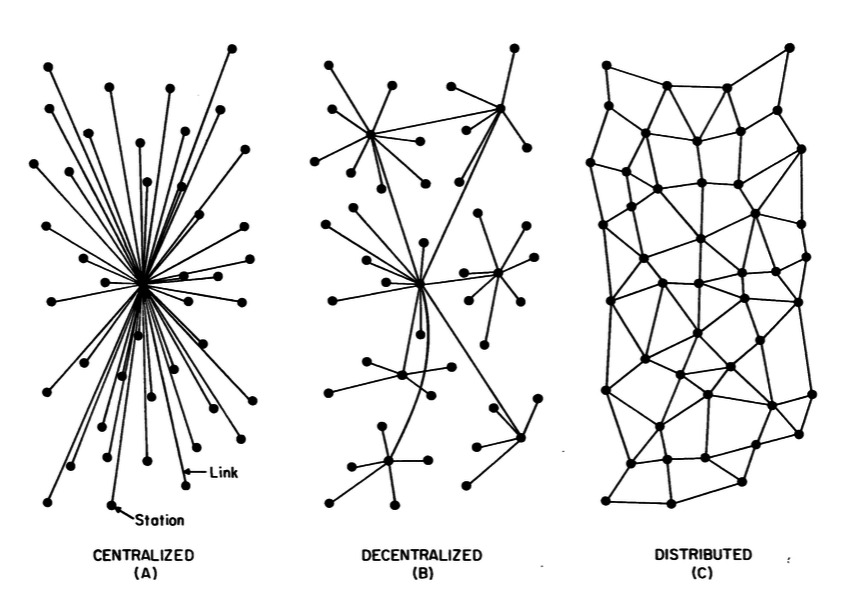
\includegraphics[width=0.8\textwidth]{figures/comparison.jpg}
  \caption{Comparison between different types of centralization.} \label{fig:comparison}
\end{figure}

When the internet was implemented as the Advanced Research Projects Agency Network (ARPANET) in 1969, it was a decentralized network of computers scattered across the United States. With the adoption of the TCP/IP in 1982, it became the internet, an interconnected network of networks.
% Todo: \cite[TCP/IP Network Administration, 3rd Edition]
In 1989, Tim Berners-Lee introduced the world wide web as a read-only means of accessing information from other computers, and the commercialization turned it into the centralized web we know today. 

In the last decade, we have seen a rise in attempts to reorganize the internet. This trend amassed attention in 2009, when the creator under the pseudonym Satoshi Nakamoto created Bitcoin, "A Peer-to-Peer Electronic Cash System" leveraging blockchain technology, followed by the Ethereum platform in 2013.
% Todo: \cite[Bitcoin whitepaper]
% Todo: \cite[Ethereum whitepaper]
% Todo: Write more about decentralization and distributed
The goal of decentralization is the separation of power from a single instance. In our case, it would be to take away control over our data from monopolies. 

Distribution takes decentralization a step further by eliminating the central control. All instances have the same amount of power.

One of the protocols that arose from this niche is the InterPlanetary File System (IPFS). IPFS is a peer-to-peer hypermedia protocol to make the web more decentralized and distributed.
% Todo: \cite[IPFS whitepaper]

Using distributed storage, in place of a centralized database, removes the single point of vulnerability and lowers the effort-to-reward balance and thus might deter malicious actors from trying to steal data.

\subsection{Homomorphic encryption}
Conventionally, encryption methods do not provide anonymity. But one could argue that in a way, anonymity is provided when the data is not readable or accessible. If an adversary manages to steal a data set while it is still encrypted, they wo not be able to infer identity or any additional information, unless they are able to decrypt it beforehand. 

Homomorphic encryption enables the arithmetic operations on an encrypted data set. They are separated into three categories:
\begin{itemize}
    \item \textbf{Fully Homomorphic Encryption (FHE)} allow multiple arbitrary operations, but have a lot of overhead and thus are expensive computationally.
    \item \textbf{Somewhat Homomorphic Encryption (SWHE)} support only selected operations to a limited number of times and are computationally more feasible.
    \item \textbf{Partially Homomorphic Encryption (PHE)} enables one type of operation any number of times.
\end{itemize}
% Todo: \cite[A Review of Homomorphic Encryption Libraries for Secure Computation]

This protects the data set from intermediate parties, making them unable to derive private data, while making it possible to work on it.

\subsection{k-Anonymity}
The above sections have shown that if a data set seems anonymous by itself, quasi-identifiers, such as ZIP code, birth date, or sex, still enable malicious actors to link individuals to their data. One of the countermeasures to this problem is providing k-anonymity. This is achieved when every query for quasi-identifier returns at least k results. A quasi-identifier is an identifier or a combination of non-identifying attributes, that can be used to link with external data sources to create new identifiers. For this, P. Samarati and L. Sweeney suggest the use of generalization and suppression.
% Todo: \cite[k-Anonymity/ A Model for Protecting Privacy.pdf]
% Todo: \cite[Protecting Privacy when Disclosing Information/ k-Anonymity and Its Enforcement through Generalization and Suppression.pdf]

Former is realized by expanding specific attributes into ranges. For instance, instead of assigning the real age, an age range is used. This results in a loss of accuracy, but a higher degree of anonymity and thus, privacy. For the latter, there are two methods of suppression. Attribute suppression removes attributes from the data set, reducing the number of possible quasi-identifiers by lowering the number of possible combinations. Record suppression, on the other hand, deletes entire entries in the data set to take out unique entries that do not meet the criteria of k-anonymity.
% Todo: \cite[Guide to Basic Data Anonymisation Techniques.pdf]

\subsection{Differential privacy}
Differential privacy can be used to prevent statistical databases from leaking private information. It is a compelling mathematical definition that is able to guarantee privacy. An algorithm is differential private as long as it disables tracing attacks, meaning that output does not show signs of a particular individual is present in it or not. Both Google and Apple have implemented differential privacy into their data collection methods.
% Todo: \cite[https://ai.googleblog.com/2014/10/learning-statistics-with-privacy-aided.html]
% Todo: \cite[https://machinelearning.apple.com/2017/12/06/learning-with-privacy-at-scale.html]

Differential privacy guarantees three qualities:
\begin{itemize}
    \item All data about an individual in the database is protected even if the adversary manages to learn auxiliary information about all other entries in the data set.
    \item Two differently differential private data sets can be combined, and the resulting data set is still differential private.
    \item It is possible to quantify the loss of privacy and information gained by the malicious actor.
    \item It can be applied to groups.
\end{itemize}

To achieve differential privacy, one basically adds noise to the data, but replay attacks can reveal actual values. To avoid this, the default noise function used is the Laplacian distribution mechanism by adding Laplacian noise. The operation can be used either on the aggregation of the user data or on the aggregated data itself.

\subsubsection{Global Differential Privacy}

If the noise function is applied to the entire aggregated raw data set, it is called global differential privacy. This works by using a noise function on the result of a query, as depicted in figure \ref{fig:global_diff}. The advantage of this model is that the resulting data set is still very accurate, but on the downside, the whole raw data set has to be available to use this function.

\begin{figure}[htpb]
  \centering
  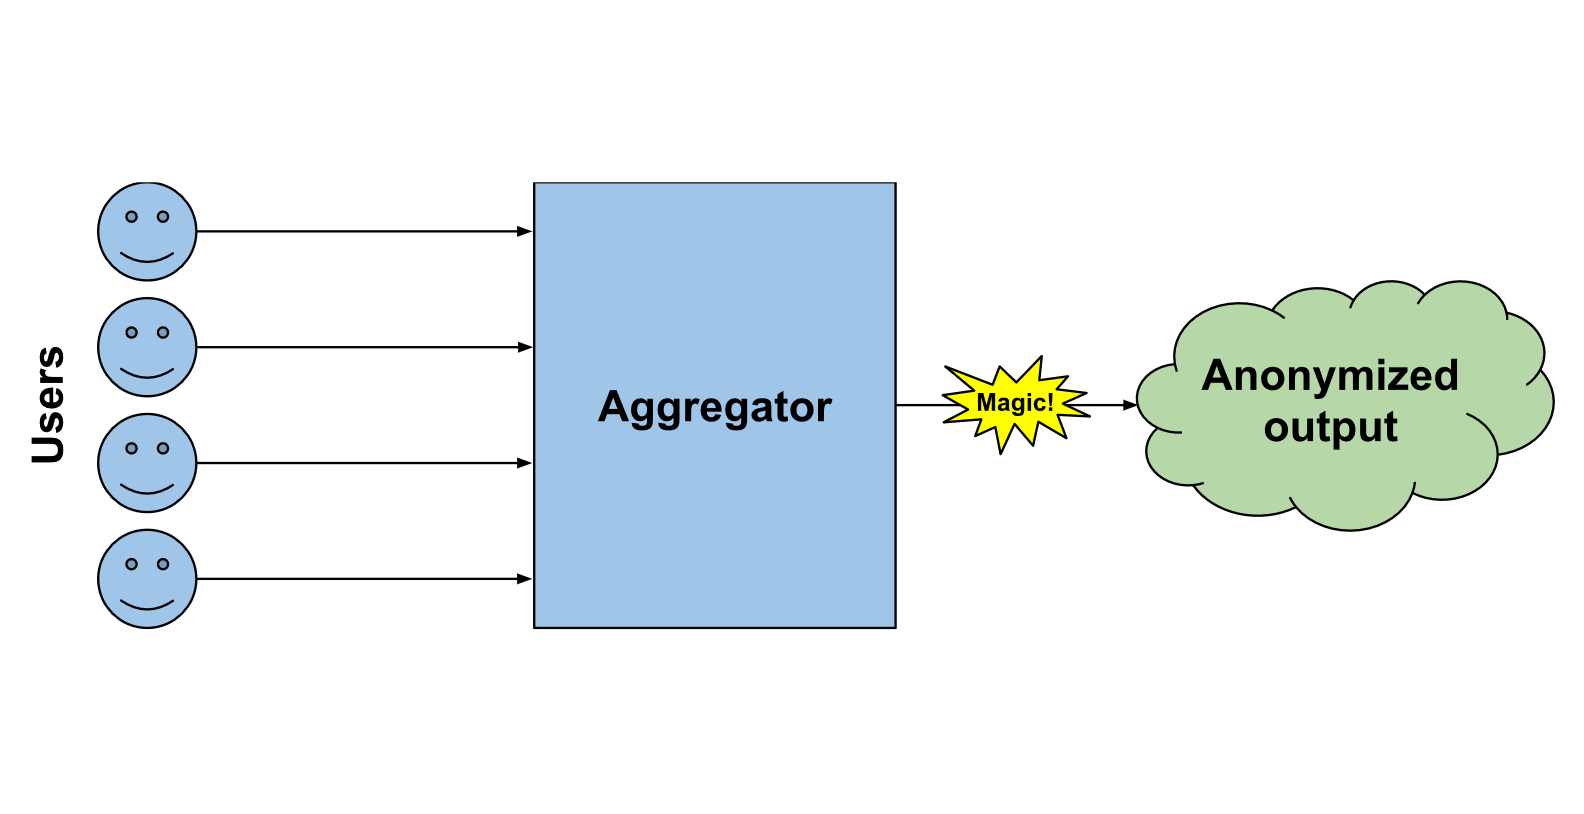
\includegraphics[width=0.8\textwidth]{figures/global_diff.png}
  \caption{Illustration of a global differential data flow} \label{fig:global_diff}
\end{figure}

\subsubsection{Local Differential Privacy}
Figure \ref{fig:local_diff} shows that differential privacy can also be used on the entries of the data. By running every entry through the mechanism, it creates a locally differential private data set. The disadvantage of this method is the much higher noise, but in exchange, the raw data itself is protected and does not require trust.

\begin{figure}[htpb]
  \centering
  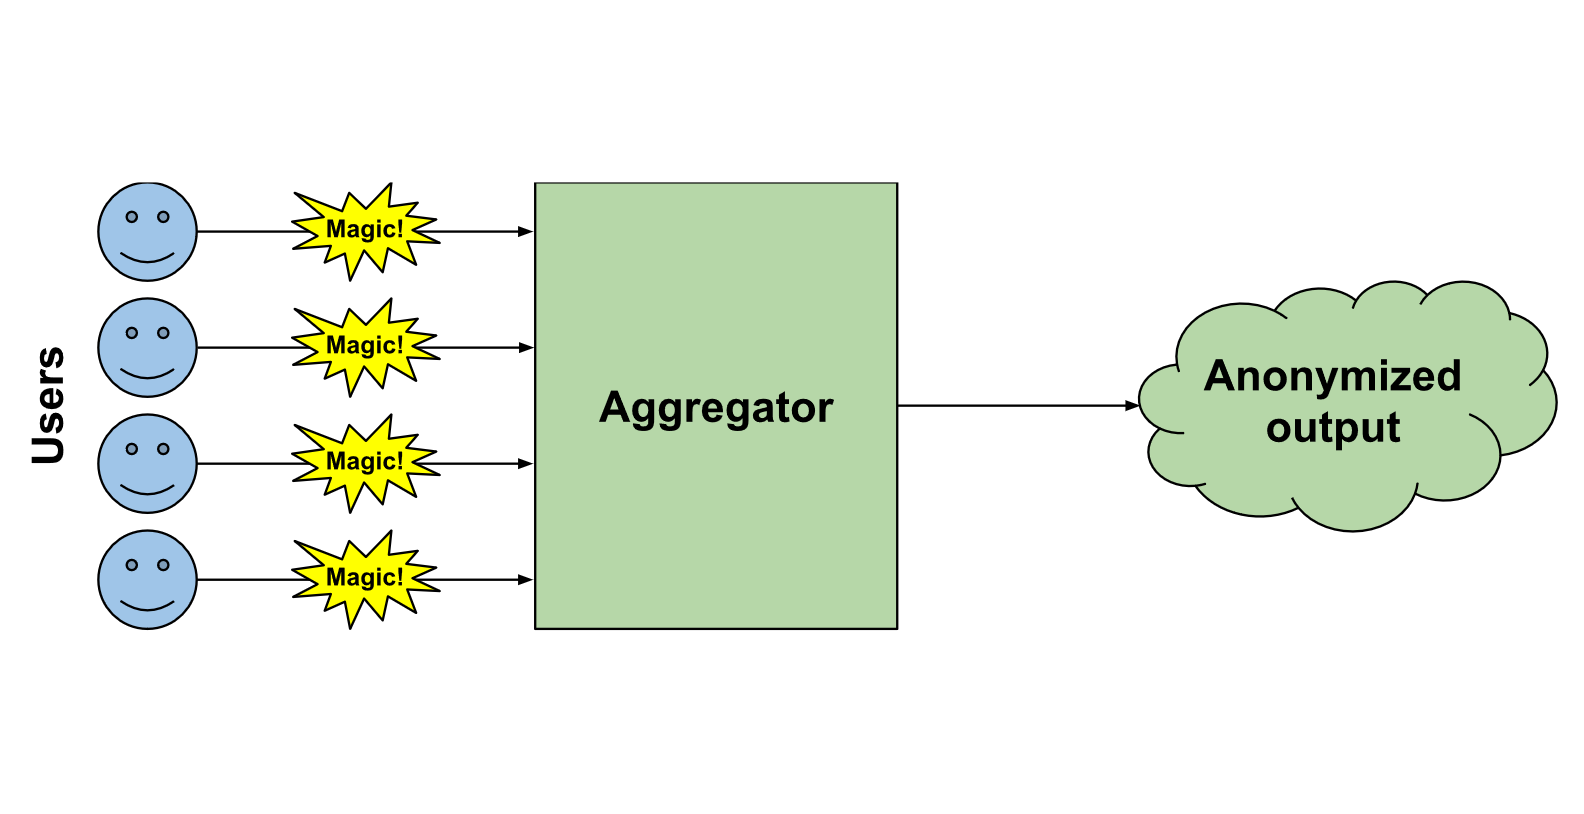
\includegraphics[width=0.8\textwidth]{figures/local_diff.png}
  \caption{Illustration of a local differential data flow} \label{fig:local_diff}
\end{figure}

A typical example of this is the coin toss. A survey asks a question that can be answered with a yes or no. The function would toss a coin and would answer the question honestly on heads and otherwise answer the question with a second coin toss, with heads resulting in yes and tails in no. 
% Todo: Not used because of focus in actual location data and dif not suitable but useful for presence

\subsection{Spatial Cloaking}
As mentioned above, spatial data can reveal a lot of sensitive information about a person. So location privacy should always be a high priority. To achieve that, there are a lot of algorithms that are used to hide the real location in a general area.

\subsubsection{Casper}
Casper
% Todo: \cite[The New Casper: Query Processing for Location Services without Compromising Privacy]
is a grid-based cloaking mechanism, that organizes the location in squares. The level of detail is ordered like a pyramid. The coordinates are cloaked by using the lower-left corner and upper-right corners as a designated area of the location. The figure \ref{fig:casper} would show the lowest level of detail with \(\langle(0,0),(4,4)\rangle\), covering the whole area, and the highest level of detail with \(\langle(0,2),(1,3)\rangle\), only wrapping a small portion of the area. To fulfill the requirements of k-anonymity, the algorithm looks for neighboring areas for other users and then spans the whole area when it finds one. For example, \(U_1\) with its cloaked area \(\langle(0,2),(1,3)\rangle\) would need the area \(\langle(1,2),(2,3)\rangle\) to satisfy \(k=4\).

\begin{figure}[htpb]
  \centering
  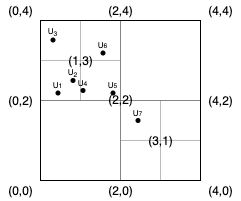
\includegraphics[width=0.5\textwidth]{figures/casper.png}
  \caption{Illustration of spatial squared areas} \label{fig:casper}
\end{figure}

\subsubsection{Interval Cloaking}
Similarly to Casper, Interval Cloaking also uses rectangular cloaking areas to hide the real locations. But instead of using neighboring squares, it uses the lower level of detail to achieve k-anonymity. Using the example from above, Interval Cloaking would span the anonymized spatial area over \(\langle(0,2),(2,4)\rangle\) to assure k-anonymity with \(k=4\) for \(U_1\).

\subsubsection{Hilbert Cloaking}
Another famous spatial cloaking algorithm is Hilbert Cloaking. This uses the Hilbert space-filling curve to map the 2-dimensional area into a 1-dimensional representation. Then it groups together points depending on the provided \(k\) because points that are in proximity on the Hilbert curve are also close to each other in 2D. Instead of using predetermined rasterization of the area, the cloaked area is spanned by the users themselves.
% Todo: \cite[A reciprocal framework for spatial K-anonymity.pdf]
% Todo: \cite[Providing K–Anonymity in Location Based Services.pdf]
% Todo: \cite[Spatial Cloaking Revisited/ Distinguishing Information Leakage from Anonymity.pdf.pdf]

